\section{Areas and Lengths in Polar Coordinates}
\begin{itemize}
    \item Suppose we have a polar curve $r= \rho(\theta)$ for $\alpha \le \theta \le \beta$.
    \item We can determine the area by partitioning the curve into $\theta_i$ and approximating each subregion as a circular segment. The area of a circular segment is:
    \begin{equation}
        A = \frac{1}{2}a^2\Delta \theta
    \end{equation}
    We can take the radius to be $r = \rho(\theta^*)$ where $\theta_{i-1} \le \theta^* \le \theta_i$. The area of each region is:
    \begin{equation}
        A_i = \frac{1}{2}\rho(\theta_i^*)^2 \Delta \theta_i
    \end{equation}
    so the total area is:
    \begin{equation}
        A = \lim_{|| P ||} \sum_{i} \frac{1}{2}\rho(\theta_i^*)^2 \Delta \theta_i
    \end{equation}
    or
    \begin{equation}
        A = \frac{1}{2} \int_\alpha^\beta \rho(\theta)^2 \dd{\theta}
    \end{equation}
    \begin{example}
        Suppose we wish to find the area of $r = 1 - \cos\theta$.
        \begin{center}
            \begin{tikzpicture}
                \draw[thick,->,>=latex] (-3,0)--(3,0) node[above] {$x$};
                \draw[thick,->,>=latex] (0,-3)--(0,3) node[left] {$y$};
                \draw[domain=0:360,scale=1.5,samples=500] plot (\x:{1-cos(\x)});
            \end{tikzpicture}
        \end{center}
        The area is then:
        \begin{align}
            A &= \frac{1}{2}\int_0^{2\pi} (1-\cos\theta)^2 \dd{\theta} \\ 
            &= \frac{1}{2}\int_0^{2\pi} (1-2\cos\theta+\cos^2\theta)\dd{\theta} \\ 
            &= \frac{1}{2}\int_0^{2\pi} \left(\frac{3}{2}-2\cos\theta + \frac{1}{2}\cos(2\theta)\right) \dd{\theta} \\ 
            &= \frac{1}{2}\left(\frac{3}{2}\theta - 2\sin\theta + \frac{1}{4}\sin(2\theta) \right)\Biggr|^{2\pi}_{0} \\ 
            &= \frac{3}{2}\pi
        \end{align}
    \end{example}
    \item We can also find the area between two polar curves $\rho_1$ and $\rho_2$. We have:
    \begin{equation}
        A = \frac{1}{2}\int_\alpha^\beta \rho_1(\theta)^2 \dd{\theta} - \frac{1}{2}\int_\alpha^\beta \rho_2(\theta)^2 \dd{\theta} = \frac{1}{2}\int_\alpha^\beta (\rho_1^2-\rho_2^2)\dd{\theta}
    \end{equation}
    \begin{warning}
        Be careful when applying this formula as it is possible the two functions can overlap between $\alpha \le \theta \le \beta$. Therefore, we always need a good idea of what's happening.
    \end{warning}
    \begin{example}
        Suppose we want to determine the area inside $r^2 = 4\cos(2\theta)$ but outside $r=1$. This gives:
        \begin{center}
            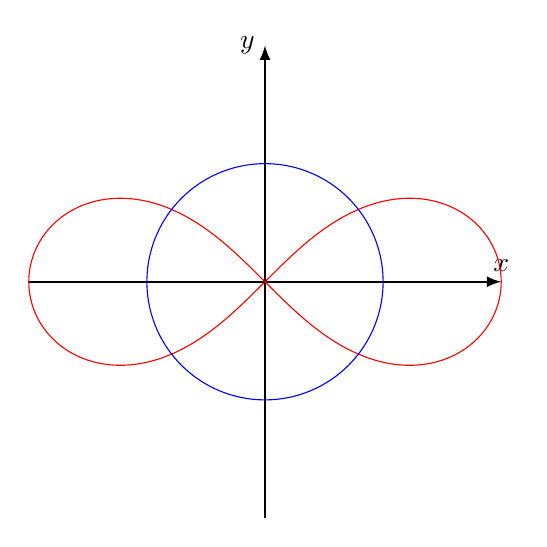
\begin{tikzpicture}
                \draw[thick,->,>=latex] (-3,0)--(3,0) node[above] {$x$};
                \draw[thick,->,>=latex] (0,-3)--(0,3) node[left] {$y$};
                \draw[red, domain=-45:45,scale=1.5,samples=500] plot (\x:{sqrt(4*cos(2*\x))});
                \draw[red, domain=-45:45,scale=1.5,samples=500] plot (\x:{-sqrt(4*cos(2*\x))});
                \draw[blue, domain=0:360,scale=1.5,samples=500] plot (\x:{1});
            \end{tikzpicture}
        \end{center}
        We first find the four points of intersection:
        \begin{equation}
            4\cos(2\theta)=1 \implies \cos (2\theta) = \frac{1}{4} \implies \theta = \pm 0.659
        \end{equation}
        or $\theta = \pi \pm 0.659$. Due to the symmetry, we only need to find the area of one half of the area we are interested in, which gives:
        \begin{align}
            \frac{1}{2}A &= \frac{1}{2}\int_{-0.659}^{0.659}(4\cos 2\theta - 1) \dd{\theta} \\ 
            &= \frac{1}{2}(2\sin 2\theta - \theta)\Big|^{0.659}_{-0.659} \\
            &= 1.277
        \end{align}
        so the area is $A=2.554$.
    \end{example}
    \item There are a few challenging examples:
    \begin{example}
        Suppose we wish to find the area between $r=\sin\theta$ and $r=\cos \theta$:
        \begin{center}
            \begin{tikzpicture}
                \draw[thick,->,>=latex] (-3,0)--(3,0) node[above] {$x$};
                \draw[thick,->,>=latex] (0,-3)--(0,3) node[left] {$y$};
                \draw[red, domain=0:360,scale=2.5,samples=500] plot (\x:{cos(\x)});
                \draw[blue, domain=0:360,scale=2.5,samples=500] plot (\x:{sin(\x)});
            \end{tikzpicture}
        \end{center}
        We know from symmetry that the intersection is at $\theta = \frac{\pi}{4}$. We notice that the contribution to the area from each curve $\rho$ is equal and \textit{independent} from each other. Therefore:
        \begin{equation}
            A = A_1 + A_2 = \int_0^{\pi/4} \frac{1}{2}\sin^2\theta \dd{\theta} + \int_{\pi/4}^{\pi/2} \frac{1}{2}\cos^2\theta \dd{\theta} = \frac{\pi}{8} - \frac{1}{4}
        \end{equation}
    \end{example}
    \item We can determine the arclength by working in parametric form. Let $x = r(\theta) \cos\theta$ and $y = r(\theta) \sin\theta$. Therefore:
    \begin{align}
        s &= \int_{\alpha}^{\beta} \sqrt{\left(\frac{dx}{d\theta}\right)^2 + \left(\frac{dy}{d\theta}\right)^2}\dd{\theta} \\ 
        &= \int_\alpha^\beta \sqrt{(r'\cos\theta - r\sin\theta)^2 + (r'\sin\theta + r\cos\theta)^2} \dd{\theta} \\ 
        &= \int_\alpha^\beta \sqrt{(r'^2\cos^2\theta + r^2\sin^2\theta - \cancel{2rr'\cos\theta\sin\theta}) + (r'^2\sin^2\theta + r^2\cos^2\theta + \cancel{2r'r\cos\theta\sin\theta})} \dd{\theta} \\ 
        &= \int_\alpha^\beta \sqrt{r^2(\cos^2\theta+\sin^2\theta) + r'^2(\cos^2\theta+\sin^2\theta)} \\ 
        &= \int_\alpha^\beta \sqrt{r^2 + \left(\frac{dr}{d\theta}\right)^2} \dd{\theta}
    \end{align}
    \begin{example}
        Suppose we want to find the arclength of $r=a(1-\cos\theta)$ from $0 \le \theta < 2\pi$. This looks like:
        \begin{center}
            \begin{tikzpicture}
                \draw[thick,->,>=latex] (-3,0)--(3,0) node[above] {$x$};
                \draw[thick,->,>=latex] (0,-3)--(0,3) node[left] {$y$};
                \draw[domain=0:360,scale=1.5,samples=500] plot (\x:{1-cos(\x)});
            \end{tikzpicture}
        \end{center}
        We have:
        \begin{align}
            s &= \int_0^{2\pi}\sqrt{r^2 + (r')^2} \dd{\theta} \\ 
            &= \int_0^{2\pi}\sqrt{a^2(1-2\cos\theta+\cos^2\theta)+a^2\sin^2\theta}\dd{\theta} \\ 
            &= a\int_0^{2\pi}\sqrt{2-2\cos\theta}\dd{\theta} \\ 
            &= a \int_0^{2\pi} \sqrt{4\sin^2\left(\frac{\theta}{2}\right)} \dd{\theta} \\ 
            &= 2a\left[-2\cos\left(\frac{\theta}{2}\right)\right]\Biggr|^{2\pi}_0 \\ 
            &= 8a
        \end{align}
    \end{example}
\end{itemize}